\documentclass[../main.tex]{subfiles}

\begin{document}
\chapter{Literature review}\label{cha:literature_review}
\section{Overview of the field}
\label{sec:overview_of_the_field}
%DONE edycyjnie: bez skrotów w stylu doesn't - zawsze pełne formy; jak chcecie myślnik, to -- w LaTeXu
A recent survey~\cite{survey2023} in the field of acoustic side-channel attacks on keyboards summarizes 31 papers, each covering a different approach. These approaches differ in what type of acoustic data is used, applied models and preprocessing techniques, target devices, and target input types (passwords, PINs, words from a dictionary, etc.).
Such a wide array of factors contributing to the overall difficulty of the task and putting different constraints on available resources, as well as a distinct lack of benchmark datasets, make the results difficult to compare.  

The easiest distinction between types of attack on keyboard acoustic emanations is whether the inference is made primarily using the sound of the keypress or the associated timing information. This timing information could refer to how much time each phase of the keystroke took or the spacing of keystrokes. It is worth noting here that keystroke dynamics have been used successfully in personal authentication~\cite{kbd-biometrics2011}. This suggests that when timing information is available, not only could the typed text be intercepted, but the identity of the typists matched to one from a database.
There is one special type of timing-based information that does not fit the framework so nicely but is important to mention because it is used in (among others) the only paper that attempts attacking unconstrained keyboard input~\cite{unconstrained2023} -- Time Difference of Arrival (TDoA).
Time Difference of Arrival is a straightforward principle -- multiple microphones with known relative locations record the same sound. Using the discrepancies in the times when a signal was received, the placement of the pressed key is estimated. This, of course, requires prior synchronization of all recording devices and a more elaborate eavesdropping setup. 

\section{Selection of important works}
%DONE 30.12.2023 wywalić te lata (daty) z tytułów
%DONE 30.12.2023 musicie konsekwentnie pisać o swojej pracy jako thesis, nie paper (drugie zdanie niżej)
\subsection{Keyboard Acoustic Emanations}
\label{sec:literature_review_keyboard_acoustic_emanations}
The seminal work in the field is "Keyboard Acoustic Emanations" by Asonov and Agrawal~\cite{og2004}. It was the main inspiration behind this thesis and the reason for many conventions used within it. The authors identified that the sound of each keystroke is composed of touch, hit, and release peaks, a notion used universally in attacks based on keystroke acoustic emanations (discussed more in Section~\ref{sec:dataset_peak_extraction}).
%DONE 30.12.2023 zawsze jak jest number po, to Section, Figure, Chapter, Table, ..., z wielkiej litery (np. zdanie wyżej)

When it comes to the type of attack they deployed -- a  connectionist neural network built with JavaNNS, which, given the sound of a single keystroke, would output its prediction of the key being pressed. The preprocessing of choice was the Fast Fourier Transform.
They manage an accuracy of 79\% on their test set. When the same network, trained on the original keyboard, is then tested on two different ones, its performance on this metric drops to 27.7\% and 21\%.

All of their experiments were conducted for 30 keys: all 26 lowercase letters, and the characters: \verb|,| (comma), \verb|.| (dot), \verb|;| (semicolon), and \verb|/| (forward slash). The training set consisted of 100 presses of each, and the test set -- 10 of each (these numbers were followed precisely in this thesis, but the set of considered keys was expanded to 43 members). 

An interesting claim that Asonov and Agrawal made is that there is no noticeable drop in performance when the distance between the keyboard and the recording microphone increases, up to their maximum tested threshold of "about 15 meters" when they used a parabolic microphone as the eavesdropping device.
Being pioneers in the field, they were also the first to explain why keys produce different sounds and discuss potential countermeasures to acoustic side-channel attacks.

% DONE: BW
\subsection{Dictionary attacks using keyboard acoustic emanations}
\label{sec:dictionary_attacks_using_keyboard_acoustic_emanations}
%TODO 30.12.2023 zmienić stylistycznie - nazwa sekcji nie jest częścią tesktu, więc pierwsze zdanie powinno lepiej wprowadzić: Berger et al. tried to preduct long words ...
%poza tym obczajcie sobie różne wersji \cite - jak \citet, \citep - one wam załatwią te wymienianki autorów odpowiednio - jak jest więcej niż 2 to się nie wymienia wszystkich w tekście tylko np. Berger et al. 
% MG: Mogę robić coś źle, ale jak chcę użyć któegoś z nich, to wszystko się psuje - oczywiście wcześniej w main dodaję \usepackage{natbib}, żeby mieć do tych poleceń dostęp. Wtedy jednak wszystkie citations się psują - nie mam pojęcia o co chodzi, może kwestia jakiejś niekompatybilności z politechnicznym szablonem

% TO_CHECK MG checked
In "Dictionary attacks using keyboard acoustic emanations"~\cite{dict2006}, Berger et al.\ try to predict long words (7-13 characters) based on a recording of a whole word and a predefined dictionary. Their main assumption is that similarly sounding keystrokes should be physically close to each other on the keyboard itself. They do not train any particular model but rather use a dictionary of words and clever narrowing of possible candidates. By creating a similarity matrix of keystrokes within a word, they are able to create constraints, for which they extract and rank possible words that satisfy these constraints.

% CHECKED - corrected citations for datasets 
\subsubsection{Datasets}
In their research, Berger et al.\ used two datasets. The first consists of 27 different words, each typed on three different keyboards using the same microphone. Because of the nature of their approach, they also used a dictionary of words created by combining two sources. The first one is \textit{SCOWL (and Friends)}~\cite{dictionary_attack_scowl} -- a database of words used for various spell-checking purposes, and the second one is CornCob~\cite{dictionary_attack_corncob} (the referenced URL seems to be outdated; there is a web page on archive~\cite{dictionary_attack_fix}, but it is impossible to verify if this is what the authors had used). Thus created word bank was used as a base of possible words, from which a ranking of candidates was constructed.

\subsubsection{Keystroke extraction}
The given recording of a word is split into 2-millisecond windows, for which their respective energies are calculated by summing their FFT coefficients. Those values are normalized to the $[0, 1]$ range. Finally, a delta vector is calculated by taking the differences between every two consecutive bins. In this vector, pairs of \textit{(surge, fall)} of energy are identified. Each such pair represents a peak in the sound of a keystroke. Two consecutive peaks are interpreted as \textit{(press, release)} of a key. They skip a press peak if the release is not found within 100ms after it.

\subsubsection{Constraint formulation}
To create a constraint, two similarity matrices are created, the first one between every identified keystroke \textit{press} and the second one between every keystroke \textit{release}. Berger et al.\ experimented with different similarities to compare signals: cross-correlation, similarities based on Euclidean distance between FFT vectors, and MFCC of two signals (see Section~\ref{sec:dataset_preprocessing} for an overview of these techniques). Five methods to aggregate the similarities between \textit{press} and \textit{release} were tested: using only one of the peaks, using whichever had the larger or smaller value, and taking their mean. They used precision and recall definitions, adjusted to their concept of constraints (more on constraints later) to assess different approaches. The conclusion was that cross-correlation and an unweighted average of similarities on \textit{press} and \textit{release} yields the best results.
These means are used to build a matrix $M$ of similarities between every pair of keystrokes within a recording of a word.


This matrix is used to create constraints, whereby a constraint means, an inferred from the mentioned matrix, relation between two keystrokes -- $K_i$ and $K_j$, expressing how far are they from each other on the keyboard. They distinguish four such relationships:
\begin{enumerate}
    \item \textit{EQ}: $K_i = K_j$ both keystrokes are from the same key;
    \item  \textit{ADJ}: $K_i \simeq K_j$ both keystrokes are the same key, or one is adjacent to the other (e.g., $Q \simeq W$, but not $Q \simeq E$);
    \item \textit{NEAR}: $K_i \sim K_j$ same as \textit{ADJ} but the distance is up to two keys (e.g., $Q \sim S$, but not $Q \sim D$);
    \item  \textit{DIST}: $K_i \nsim K_j$ which means that those keys are not \textit{NEAR} to each other (e.g., $Q \nsim P$).
\end{enumerate}

They introduce \textit{BestFriendsPickPolicy}, which was the best method to assess constraints from a given similarity matrix. It is calculated in the following way: let $rank(i, j)$ be the position of keystroke $j$ in $M_{i*}$ row of similarity matrix (without $M_{ii}$), sorted in decreasing order. Then, based on the sum $rank(i, j)$ + $rank(j, i)$, the constraint is chosen. If the sum is smaller than 3, it is considered \textit{EQ}; if it is equal to 3, it is \textit{ADJ}; if it is equal to 4, it is \textit{NEAR}, and for values bigger than 4, it is considered \textit{DIST}.

\subsubsection{Constraints evaluation}
The problem is that a particular word has a distinct set of constraints, but the opposite is not true. What is more, even one false constraint can cause the searched word to not be detected. Thus, an evaluation of constraints and their refinement is needed.

Without getting much into detail, they create many subsets of constraints (with probability $p$ that constraint $\xi_m$ will be included), and for each of them, create a list of words from the dictionary that are consistent with those constraints. With some smart data structures and optimization, they avoid very time-consuming computations.

Finally, all words in the dictionary are sorted in decreasing order of the number of occurrences in different lists. That final ordering calculated with sufficiently many lists should ensure that the original word will be near the top.

\subsubsection{Results}
Because of the form of the attack, they calculated the success ratio as the frequency of the correct word appearing in the top N words from their candidate list. They measured different top sizes and achieved a success rate of 73\% for the top 50 words, as well as almost 90\% for the top 100 words.

One of the more interesting results is that the success rate increased with the number of repeated characters in the word. If at least two \textit{EQ} constraints existed in the original word, the success rate jumped to over 90\% even for the top 25 words.

Another insight is that the length of the original word impacted the success rate. The longer the word was, the better results their technique obtained, yielding over 90\% success rate for the top 25 words if the considered word was 13 letters long.

\subsubsection{Observations and shortcomings}
Even though Berger et al.\ conducted full research on the topic of reconstructing a word from its recording, the rather small size of their dataset casts a shadow on their work. They state that they recorded 27 different words on three different keyboards, resulting in a total of 81 different recordings.
Restricting the targets to longer words, which must come from a dictionary known a priori, is a significant limiting factor, which must be taken into account when comparing the results to other works.

Another issue is that their description of keystroke extraction lacks many important details. More precisely, they did not specify the procedure of extracting \textit{surge}{\textbackslash}\textit{fall} moments from processed recording. This detail makes their work less reproducible for future researchers.

Even though finding the correct word within the top 50 candidates with a 73\% success rate drastically reduces all possible \textit{long} words, it is far from saying that this method reconstructs a word from a recording. For many use cases, a much higher accuracy in picking up the correct word is needed.

Despite these problems, this work was found essential to include in the review due to two unique traits. Firstly, the approach does not need any training or information about the typist. Secondly, the way recordings are processed and keystrokes extracted is keyboard-independent, which should allow for strong generalization of the attack.


\subsection{Content Reconstruction using Keystroke Dynamics: Preliminary Results}
\label{sec:content_reconstruction_using_keystroke_dynamics_preliminary_results}
"Content Reconstruction using Keystroke Dynamics: Preliminary Results"~\cite{content_reconstruction_2014} tries to attack keyboard acoustic emanations from a completely different direction, using only the duration of keystrokes. Using different classification techniques and some NLP procedures, they tried to re-create a natural language sentence. They also created a huge dataset consisting of durations of different keypresses of over 30 participants. The paper is unique in how little information its techniques require on input (one number per one keystroke), but unfortunately, results show that this approach is impractical (at least at this stage of research). Nevertheless, this work gave a different perspective on acoustic side-channel attacks and possible avenues to explore.

\subsubsection{Dataset}
Liang Wu and Patrick Borus describe keystroke dynamics as behavioral biometrics depicting one's typing style, making it possible to identify the typist to some extent. Several different features can be taken into account when discussing keystroke dynamics. The researchers decided to use key press duration exclusively, as it was more stable than the other timing feature, which was inter-key latency. The duration is expressed as a whole number of milliseconds. They included the following 33 keys in their dataset: all letters, space, backspace, enter, comma, period, left shift, and right shift. They use all of the keys to train models, but later in the paper, they assume that only 27 classes exist: letters and  \textit{space}.

For the purposes of this paper, a diverse dataset of keystroke durations was created. To record it, every one of the 31 participants used \textit{BeLT} software, developed at \textit{NISLab}. Every participant typed, on average, over 75000 keystrokes, creating a dataset of over 2 million pairs of \textit{(key, duration)}. They did not provide any specific information about the keyboards used. One can guess that because each participant had to install software on their private computer, each participant also used their own keyboard to create a dataset.


They also used a dictionary of 10000 of the most popular English words; the source is unknown. 
\subsubsection{Used techniques}
The original dataset is divided into train and test sets with a ratio of 2:1. To classify characters, four different methods were proposed:
\begin{enumerate}
    \item \textbf{Gaussian distribution} -- for every class, standard deviation $\sigma$ and mean $\mu$ of the duration are calculated. Every new keystroke with duration $x$ is assigned to the class for which the value of $f(x, \mu, \sigma) = \frac{1}{\sigma *\sqrt{2\pi}} * e ^{\frac{1}{\sigma *\sqrt{2\pi}}}$ is the highest.
    % the class is chosen based on the distance PDF with such equation $\frac{1}{\sigma *\sqrt{2\pi}} * e ^{\frac{1}{\sigma *\sqrt{2\pi}}}$, where $\mu$ and $\sigma$ are calculated separately for every class, where higher values are favored. 
    % proponowane przepisanie:
    % for every key, standard deviation $\sigma$ and mean $\mu$ duration are calculated. Every new keystroke with duration $x$ is assigned to the class for which the value of f = $formula here$ is the highest
    \item \textbf{Distance} -- similarly to Gaussian distribution, but with a minimum value of the following expression determining the assigned class $d = \frac{|x - \mu|}{\sigma}$.
    \item \textbf{k-NN} -- with flexible $k$. The final class of a keypress in question is the majority class in a set of instances for which duration is identical to the considered keypress.
    % question: transfer_function == activation_function
    \item \textbf{Back-Propagation Neural Network (BPNN)} -- with one hidden layer consisting of 30 neurons and Tan-Sigmoid function and the output layer of 6 neurons (each neuron represents a bit when encoding the predicted class as a binary number). \textit{Scaled conjugate gradient back propagation algorithm} is used as a learning procedure.
    % wywaliłem kawałek o linear activation function na końcu, bo to tylko ich bad practice - wiemy, że linear activation functions nie mają za dużo sensu - linear combination of linear combinations...
\end{enumerate}
For later stages of the attack, a probability of belonging to a particular class is needed; thus, some transformations of established methods are needed. For the \textit{distance} method, the normalized reciprocal of every class is calculated. For \textit{Gaussian distribution} similarly, the probability of belonging to a particular class is equal to its probability density, normalized over probability densities of all classes. Regarding the \textit{k-NN}, the probability is equal to the ratio of instances with the particular class to the size of $k$. % for BPNN they did not gave anything

\subsubsection{Attack scenario}
\label{subsubsec:dynamics_attack_scenario}
The authors assume that the attacker acquired keypress timing data from, e.g., visual or acoustic eavesdropping on the victim. The next step is to reconstruct the sequence of characters from the durations of each keystroke. The attacker uses pre-trained models or other techniques to achieve it. The reference data needed to perform training can come from one of 3 sources:
\begin{enumerate}
    \item The attackers -- they can perform recordings themselves.
    \item General data -- a dataset consisting of keystroke dynamics different people could be composed, from different attacks, etc.
    \item The victim -- the least possible option, where the attacker could get keystroke dynamics of the victim.
\end{enumerate}
The choice of reference data impacted which part of the dataset techniques was trained.
The scenario considered in "Content reconstruction..." was where 1 of 31 participants was chosen as the attacker, another one as the victim, and data of the rest of them was used as general reference data. The victim was asked to type and record with \textit{BeLT} one grammatically correct English sentence, which would then become the target of the attack. Naturally, the information about its characters was removed.

\subsubsection{Pattern recognition}
It is very important to divide the input sentence into consecutive words correctly. Using established techniques, the researchers begin with classifications of durations corresponding to \textit{space} and \textit{not-space}. None of their models exceeded an 81\% accuracy, which is exactly the fraction of \textit{not-space} keys in the training dataset. In other words, these models could not beat a trivial model that always returns the decision "\textit{not-space}" -- they needed to change their approach.

Instead of this "space classification", they create a list of all possible words that have the same length as the number of durations between \textit{spaces}, whose locations are given beforehand. The dictionary of 10000 English words mentioned earlier is used to remove incorrect words. Final words are ordered based on probabilities of characters and categorized as parts of speech. Then, the researchers try to recreate the sentence, using the relations between different POS words and where they belong in English sentences. They also base their decision on the "meaningfulness" of the sentence. Unfortunately, the previous step had been done manually; thus, reproduction is impossible. Finally, after five partial guesses and feedback from the victim (no particular information about the form of the feedback or what the researchers mean by "partial" was provided), the researchers were able to reconstruct the sentence that the victim wrote before the attack. 

\subsubsection{Results}
Unfortunately, the results of their experiments show that such an arrangement of attack is rather impractical. At the very first stage, classification of \textit{space}, their best model (BPNN) achieved 72\%, whereas their baseline was 81\%. Thus, their best model did not achieve even the baseline. To proceed with experiments, they had to make unrealistic assumptions that the location of spaces was known at the beginning of the attack. The step of sentence reconstruction based on probabilities of word occurrence and their POS tag took them \textit{22 working hours}, and finally, after their fifth partial guess and feedback from the victim, they were able to guess the sentence. They estimate that without the victim's feedback, the whole procedure would take 40 working hours.
The best accuracy of general recognition of a character was achieved by k-NN with 17.83\% accuracy.

One of the most exciting results is that, according to their experiment, there is no substantial difference between using the victim's, general, or attacker's reference data. They introduce a simple grading model: for every word in the original sentence, its score is calculated by taking its position in a list and dividing it by the length of the list (the list is ordered by descending probability of occurrence of the word, and the list has only words with a particular POS tag). Such scores are calculated for every word in the sentence and for every classification technique. At the end, the average of all scores is taken. Calculating the scores for every reference data yields the following results: victim's reference = 0.46, general reference = 0.46, attacker's reference = 0.45.

\subsubsection{Conclusions}
This paper showed a different approach to tackling acoustic side-channel attacks. It uses different features one can exploit to reconstruct keystroke sequences -- not relying on the signal's content, but rather on the press duration of different keys. 

They also leveraged the properties of the English language to further increase their chances of success, which is another thing to consider when attacking natural language inputs. Part of speech tagging and its relationship to the position in the sentence is one such example, but a large predefined dictionary of correct words can also immensely help in the task of sentence reconstruction.

At the same time, there are several issues with this paper. First of all, some of their results are derived from experiments conducted on insufficiently sized samples. For instance, the conclusion about there being almost no difference in performance when other types of reference data are used (the types mentioned in Section~\ref{subsubsec:dynamics_attack_scenario}), is based on only one performed attack scenario, which had only one sentence with 21 words. It is a tiny sample, which puts the validity of the experiment into question.

Such a small sentence size and only one sentence that tested this attack scenario are mainly related to another issue, which is their step of sentence recognition from POS-tagged, most probable words. Not only was it made by hand, but they also needed five partial questions to the victim and his feedback to reconstruct the sentence. On top of that, it took them 22 working hours to complete. 

They are aware of that issue and write that plenty of things need to be improved in this research. Most of those simplifications were made to get to the final results, including more simplifications such as prior knowledge about \textit{spaces} location, and knowledge about the victim's alphabet (not using some keys in the tested sentence)

% DONE: PK
\subsection{Skype \& Type: Keyboard Eavesdropping in Voice-over-IP}
\label{sec:skype_type_keyboard_eavesdtopping_in_voice_over_ip}
"Skype \& Type: Keyboard Eavesdropping in Voice-over-IP"~\cite{skype2019} is a sequel to 2017's "Don't Skype \& Type! Acoustic Eavesdropping in Voice-over-IP"~\cite{skype2017}, published by a group of 5 researchers, 4 of which were also authors of the original.

\subsubsection{Realistic assumptions}
What sets these works apart is the realistic assumptions in the proposed threat model. Namely, the victim is assumed to be typing on a keyboard during an ongoing VoIP conversation with the attacker. There is no tampering on the victim side, meaning both their physical equipment (keyboard, microphone) and their software are operating within the expected norms. In other words, the attacker has no other information than the raw audio signal received through the VoIP software. The audio is assumed to consist of a single-channel (mono), which eliminates the possibility of approximating the relative locations of pressed keys.

The authors consider three possible "victim configurations":
\begin{enumerate}
    \item The victim's microphone is built into the computer.
    \item The victim is using an external microphone connected to
    the computer (e.g., a headset).
    \item The victim is using an external device to connect to the
    VoIP call. The microphone is built into the external device
    (e.g., talking on the phone that is in the proximity of the
    keyboard).
\end{enumerate}

In building the dataset, the authors involve 12 unique participants
covering a broad range of 11 different models of keyboards. The participants
have varied typing speeds, which, in the case of faster typists, poses an extra
challenge to the data segmentation stage due to the increased possibility of
overlapping keystroke sounds.

Finally, the authors distinguish three levels of difficulty with respect to how much prior preparation is available to the attacker (in both papers referred to as "Profiling scenarios"):
\begin{enumerate}
    \item \textsc{Complete Profiling}: The attacker owns labeled acoustic samples of the victim typing on the target device. This can be a result of prior interactions during which the victim unwittingly typed and sent messages directly to the attacker or through a channel to which the attacker had simultaneous access. The length of such samples is limited to a few hundred characters.
    \item \textsc{User Profiling}: The attacker owns labeled acoustic samples of the victim typing on a different device of the same \emph{type} (e.g., a different keyboard model). This type of data can be obtained through social engineering methods. A model trained on a particular model of keyboard is usually found to perform much worse on a different model of keyboard, even if all other details of the classification task given to it remain the same~\cite{og2004}.
    \item \textsc{Model Profiling}: The attacker has no prior knowledge of the victim's device, their typing style, or what they typed. This is the most complex scenario, for which the authors make the assumption that the attacker is in possession of a database of various keyboards' acoustic sounds. Thus, carrying out a successful attack simplifies to the \emph{Complete Profiling} case, with an added initial step of finding a match in the database. In case of no such match, the attacker must either be satisfied with a lower-accuracy equivalent from the database or try to obtain more information via social engineering or fingerprinting techniques.
\end{enumerate}

\subsubsection{Feature extraction}\label{sec:skype_feature_extraction}
Getting from raw acoustic data to a vector of features is done in 3 steps: Segmentation, Slicing, and Feature Extraction. During Segmentation, the algorithm steps through a normalized waveform in 10ms segments, computes the energy of each segment, and, if above a certain threshold, marks the segment as an "event", i.e., a keystroke. During Slicing, up to 100ms of sound are extracted from the start of each event (the duration can be lowered to prevent overlap). Finally, mel-frequency cepstral coefficients are derived from each region. Cepstral coefficients and FFT are listed as explored alternatives, but apparently, both gave worse results than MFCC. This was determined by training a Logistic Regression classifier on a simplified dataset consisting of 10 samples of 26 keys of the English alphabet.

The authors of \emph{S\&T} distinguish only two peaks, press and release. This is somehow a simplification of the model established by Asonov and Agrawal, who observed that the press peak can be further broken down into touch and hit peaks, cutting out the brief silence between the finger touching a key and the key hitting the keyboard plate~\cite{og2004}. This nuance is not commented on in \emph{S\&T}. However, from the experience of visually comparing waveforms across the datasets created for this thesis, this distinction between touch and hit peaks is not always clear. In any case, in \emph{S\&T}, only the press peaks are consumed by the machine learning model (the release peaks are discarded).
% DONE: PK: describe segmentation 10ms window & 100ms peak length -- theorize on whether
% the touch peak is included or not

\subsubsection{Results}
The number of different scenarios and configurations tested in the paper is vast,
as is the scale of the results. We shall only mention those results that co-align with
our topic and are the closest to being faithful benchmarks for our own evaluations.
That said, curious readers are encouraged to read the original work to get to the
finer details of the authors' findings and conclusions.

One of the interesting conclusions in the paper is the lack of a significant difference
between hunt \& peck and touch typing styles. The difference is said to be only
0.80\% on average, in favor of h\&p typists. As for the best top-1 accuracies obtained,
they range pretty wildly based on a few factors. Note that the numbers below correspond
to the touch typing style (the authors do not specify a similar list of concrete values
for h\&p). To roughly convert to h\&p accuracies, 0.8\% would need to be added:
\begin{center}
    36.81\%, 38.92\%, 48.08\%, 52.67\%, 59.8\%, 73.3\%--83.23\%
\end{center}
These accuracies were obtained on different keyboards, and, perhaps more importantly,
different microphones. Here are the corresponding top-5 results:
\begin{center}
    65.81\%, 68.02\%, 79.72\%, 79.56\%, 83.5\%, 94.5\%--97.1\%
\end{center}

The results obtained by \emph{S\&T} fall very close to the ones obtained in this work,
as explored in Chapter~\ref{cha:results}.

% triangulation-based
% DONE: PK
\subsection{Identifying keys using acoustic emanations from keystrokes}
\label{sec:identifying_keys_using_acoustic_emanations_from_keystrokes}
"Identifying keys using acoustic emanations from keystrokes" is a recent work by Nakken, which boasts an 87.1\% accuracy of predicting a random
keystroke using a four-microphone setup and TDoA~\cite{nakken2023}. Noteworthy
is the high-grade equipment used (192kHz cardioid XLR microphones connected to
an external audio interface), which doubtless had its hand in the quality of
the final results.

\subsubsection{Methodology}
The only prerequisites needed to perform classification are feature vectors
for each key type. These feature vectors are extracted from labeled training
data. Then, classifying a keystroke is as simple as extracting
its features in the same way as during training and comparing those features
against the ones in the database, returning the closest match. These are the
surface-level principles behind any TDoA method; more details will follow
in upcoming sections.

\subsubsection{Physical setup}
The microphones were placed close to the keyboard, situated near each of its
corners. Care was taken not to place them on the same table surface as the
keyboard itself to prevent traveling vibrations from influencing the audio
readings and providing an unfair advantage. A photo of the rough setup is
provided, as seen in Figure~\ref{fig:nakken2023_setup}.

\begin{figure}[h]
    \centering
    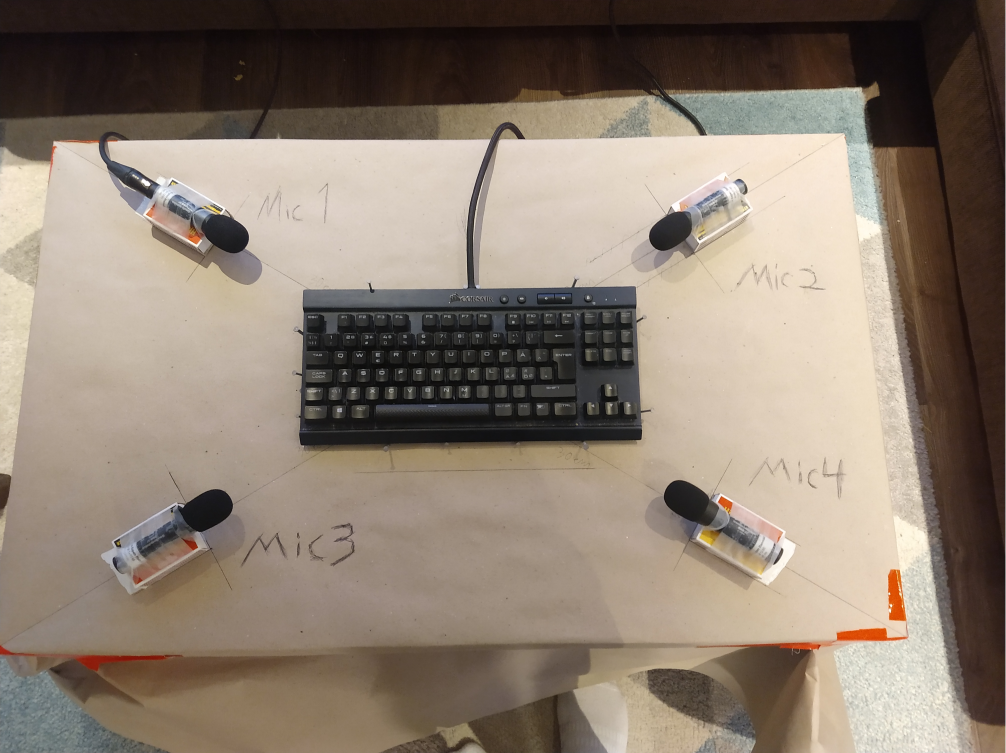
\includegraphics[width=0.5\linewidth]{figures/nakken2023_setup.png}
    \caption{Physical setup used for recording (source:~\cite{nakken2023})}
    \label{fig:nakken2023_setup}
\end{figure}

\subsubsection{Dataset construction}
Not unlike most researchers of keyboard acoustic attacks, Nakken records their own
dataset, the details of which are succinctly detailed in the paper. He is the
sole typist contributing to the dataset, which could call into question whether
the collected data is subjected to a typing style bias, but it is remarked
earlier that triangulation-based methods are not as dependent on behavioral
patterns as machine learning methods. The reason for that seems intuitive
-- triangulation utilizes only TDoA, which does not carry any information about
the timbre of the keystroke (which is affected by how a person presses each key).
Conversely, machine learning relies exclusively on the timbre to perform the
classification.

At the start of each recording session, a point equidistant to every microphone
is found, and the table is tapped there three times. This is done for the
purposes of later synchronization of all four recordings (see Section~\ref{sec:nakken_feature_extraction}).

The dataset was pretty minimal in terms of variety, comprising only the
keys for English letters "a" to "z", the spacebar, and the comma. A total
of 4 dataset parts were recorded:
\begin{enumerate}
    \item \textbf{Individual presses} -- Pressing each key individually 50 times.
    \item \textbf{Words} -- Typing eight predefined words, each repeated three times.
    \item \textbf{Sentences} -- Typing three predefined sentences, once each.
    \item \textbf{Touch typing} -- Same as \textit{Sentences}, but touch
    typing instead of hunt \& peck.
\end{enumerate}
With the exception of \textit{Touch typing}, all keystrokes were made in slow
succession (1-2 second delay between presses) using the index finger. Note that
since TDoA methods do not care about the timbre of the sound, there is no need
to perform any audio extraction and, therefore, no need for logical separation
of peaks. Nakken comments that each keystroke was conducted in "one swift motion",
with no intent to keep the press and release events separate.

Only \textit{Individual presses} are used for training and testing classifiers.
The remaining 3 dataset parts are provided only as an additional tool for future
researchers.

\subsubsection{Feature extraction}\label{sec:nakken_feature_extraction}
The goal of feature extraction is to turn audio signals from 4 microphones
into a single feature vector, whose goal is to uniquely identify the key that
was pressed.

First, it must be ensured that the four signals are synchronized correctly. It is
known that each recording begins with three peaks corresponding to taps that were made
in a spot equidistant to each microphone. Ignoring slight inaccuracies, these taps
should match perfectly for all signals. The offset between each of the 6 pairs of
recordings is calculated using cross-correlation, and the signals are aligned
by padding them with 0s at the beginning or the end.

Then, segmentation is done on each of the signals, giving the relative time of every
keystroke, as perceived by each microphone. This procedure is done using very similar
principles of stepping through the waveform and comparing energy with some threshold
as already seen in~\cite{skype2019} (see Section~\ref{sec:skype_feature_extraction}).

Finally, for each keystroke, the differences in relative timing between all pairs
of microphones are computed, again using the cross-correlation function, and returned
as a 6-element vector.

\subsubsection{Training and testing}\label{sec:nakken_training_and_testing}
During training, for every key, training data consisting of multiple recordings of
that key being pressed is transformed into a single "reference vector". A reference
vector is created simply by extracting feature vectors from each recording of the
same key, and taking averages of each of their six components.

Once training is complete, a prediction of an unlabeled signal is made by extracting
its feature vector, comparing it against each of the 28 reference vectors, and selecting
the key whose reference vector was the most similar. A comparison between two feature
vectors is done by summing absolute values of pairwise differences between the vectors'
components, with lower values indicating stronger similarity. This similarity function
is referred to as \textbf{Sum of all TDoA differentials} in the original paper.
A relaxed version called \textbf{Sum of the three lowest TDoA differentials} is also
proposed, which works exactly like the former method, except it returns the sum
of only the three lowest differences. This is supposed to filter out high differentials
which might be caused by inaccuracies.

\subsubsection{Dividing the dataset and related ambiguities}
Only 50 examples per key are considered, which is not a great amount of data.
To circumvent this limitation, Nakken uses a simple technique akin to 2-fold
validation: The training is done in 2 rounds. In the first round, a classifier
trains on the first 25 examples, and the remaining ones are used as a test set.
In the second round, the roles of examples are reversed -- the classifier learns
on the last 25, and testing is done using the first 25.

Unfortunately, this explanation is missing some important details -- how
exactly is this 2-round training process conducted? Two interpretations
that come to mind are:
\begin{enumerate}
    \item [Interpretation 1]
    \begin{enumerate}
        \item An empty classifier is initialized.
        \item The classifier is \textbf{trained} on the first 25 examples,
        producing reference vectors.
        \item The classifier is \textbf{tested} on the last 25 examples.
        \item The classifier is \textbf{trained} on the last 25 examples,
        \textbf{combining} new vectors with the pre-existing ones.
        Since all reference vectors are averages taken from the same
        number of elements, "combining" could simply mean taking the
        average of those two averages. This is purely speculative,
        as Nakken does not mention this operation anywhere in the paper.
        \item The classifier is \textbf{tested} on the first 25 examples.
        The results are obviously unreliable, because the testing data has
        been leaked in b).
    \end{enumerate}
    \item [Interpretation 2]
    \begin{enumerate}
        \item An empty classifier is initialized.
        \item The classifier is \textbf{trained} on the first 25 examples,
        producing feature vectors.
        \item The classifier is \textbf{tested} on the last 25 examples.
        \item A second empty classifier is initialized.
        \item The second classifier is \textbf{trained} on the last 25 examples,
        producing \textbf{new} feature vectors.
        \item The second classifier is \textbf{tested} on the first 25 examples.
    \end{enumerate}
\end{enumerate}

Since Interpretation 1 leads to a blatant violation of basic machine
learning principles, believing in Interpretation 2, or a similar version of it,
inspires more confidence in the validity of these experiments. However,
when describing this 2-round process, the original paper does not mention
resetting or initializing a fresh classifier after round 1. The omission of
this detail seems like a significant oversight.

Another important detail that is left out is what method was used to aggregate
the results from both rounds of testing. The paper presents a single accuracy
score for each key, but these scores had to be derived from pairs of numbers,
somehow. Whether it was an average, a minimum, a maximum, or something entirely different, is not commented on. This, in conjunction with the aforementioned interpretation ambiguity, makes it very difficult to grasp the true meaning of the final results.

\subsubsection{Results}
The results are split based on the similarity function used (see Section~\ref{sec:nakken_training_and_testing}):
\begin{description}
    \item [\textbf{Sum of all TDoA differentials}]
    \begin{itemize} \item[]
        \item Total Accuracy: \textbf{67.8}\%
        \item Accuracy per key (min, avg, max): \textbf{28\%} -- \textbf{67.7\%} -- \textbf{98\%}
    \end{itemize}
    \item [\textbf{Sum of the three lowest TDoA differentials}]
    \begin{itemize} \item[]
        \item Total Accuracy: \textbf{87.1}\%
        \item Accuracy per key (min, avg, max): \textbf{45\%} -- \textbf{86.7\%} -- \textbf{100\%}
    \end{itemize}
\end{description}

% DONE (tylko ta sprawa z mu): MG
% keep \mu in mind - FIX IT, somehow - used \textmu
\subsection{Auditory Eyesight: Demystifying \textmu s-Precision
Keystroke Tracking Attacks on Unconstrained 
Keyboard Inputs}
\label{sec:auditory_eyesight_demystifying}


The latest paper in this assortment, "Auditory Eyesight: Demystifying 
\textmu s-Precision Keystroke Tracking Attacks on Unconstrained Keyboard Inputs"~\cite{unconstrained2023},
can be seen as a new significant step in the study of attacking keyboard acoustic emanations.
Tu et al.\ are the first to claim to have devised a process capable of identifying
arbitrary inputs based on the sounds of typing. This would include any
special characters, capitalization, and handling scenarios when the typist
deletes a previously entered character. This flexibility is enabled by the
core principle of the schema -- precise localization of keys based on the
time difference of arrival (TDoA) of the keystroke sound. 
"Auditory Eyesight\ldots{}" reports many impressive results, but a closer inspection
of the methodology and datasets makes a reader look at them in a less favorable light
(see Section~\ref{sec:results_and_shortcomings}).

\subsubsection{Technique overview}
The microphone array used (ReSpeaker 6-Mic) holds 6 microphones, arranged 
so that they form the vertices of a hexagon. In all of the experiments, two pairs
are selected from them to perform the recordings. Microphones from one pair are always 
selected to be spread out more horizontally, the other -- more vertically.
The convention established by the authors is that the difference between arrival times
to microphones of the "horizontal pair" is labeled as $\Delta T_1$ and the "vertical pair"
as $\Delta T_2$
This way, the TDoA captured by the first pair helps to identify the "row" in which
the pressed key was situated, while the second one -- the key's horizontal position.
No discretization is utilized, the notion of a keyboard row is used here to
provide a simplified differentiation between keyboard axes.
All four microphones are recording at a 44.1 kHz sample rate.
However, to achieve the necessary precision, the signal must be upsampled
and synchronized. Three phases of this process have been outlined by the paper's authors.
They are presented in more detail in Section~\ref{sec:approach_details}.


With two pairs of microphones, each keystroke has two associated TDoA values
($\Delta T_1$ and $\Delta T_2$). One can think of them as the estimated coordinates
of the pressed key. Tu et al.\ note that a key on a keyboard is not a single point
and that the sound it produces does not always originate at the same location, especially
when a human is doing the typing.
Therefore, what they are trying to accomplish is to build a type of map of the keyboard, with
concentrated clusters of points in the $(\Delta T_1, \Delta T_2)$ coordinate system representing
keys.
When an attack is launched, the location of each perceived keystroke is estimated in the same way
as during the construction of the keyboard map. Euclidean distance is used to calculate the distance
between the newly created point, and the mean values of each cluster. The attacked sample is labeled
as the key for which this distance is minimal. Figure~\ref{fig:auditory_eyesight_keyboard_map} is an intuitive visualization taken from a presentation  accompanying
"Audiotry eyesight\ldots{}"\cite{presentation_unconstrained2023} illustrating the final product of the process.
Concentrated clusters of points can be thought of as a representation of each key on a keyboard. 

\begin{figure}[H]
    \centering
    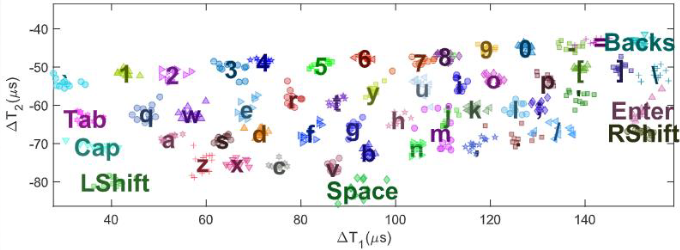
\includegraphics[width=0.8\textwidth]{figures/auditory_eyesight_keyboard_map.png}
    \caption{Visualisation of the "keyboard map" obtained by estimating keystroke locations}
    \label{fig:auditory_eyesight_keyboard_map}
\end{figure}


\subsubsection{Approach details} \label{sec:approach_details}

The \underline{i}nitial round consists of several steps.
First, the signal is filtered with a zero-phase, high-pass Butterworth filter
\cite{aremu2013-butterwotrth-filter} set to pass frequencies from 1 kHz. 
The filtered signal is upsampled with a rate of 40 and interpolated,
leading to a new sample rate of 1761 kHz.
After this process, a single unit represents 0.5686 $\mu$s. 
On this fine-grained signal, outliers are eliminated.
This itself is a two-stage process, consisting of removing keystroke recordings for which
TDoA values are not within 3 standard deviations from the median 
\cite{leys2013detecting_outliers}.  These filtered examples
are then filtered down more, by preserving ones with values from
a percentile range $[s\%, (100-s)\%]$ ($s$ is stated to be from the
range of [2, 10] -- examining the source code reveals that values
of 2, 5, and 10 were used, seemingly arbitrarily;
and once a range of [5\%, 98\%] was specified).
% source of the 5, 98: https://github.com/auditoryeye/auditoryeye_artifact/blob/333e8c5480ff0f6db7c0f0012a6c38a7f4126693/04_additiontestcase_angle02/YZProcessing05_statistics_remoutlier.m#L89C39-L89C45
Now the reference point of the keyboard (its center) can be estimated,
by taking the mean of all positions of estimated key locations obtained
from non-outlier TDoAs.

Round 2 (referred to in the paper as B-round, for \underline{b}ounding the range)
begins by aligning the signals received by two microphones forming a pair, by
padding them with zeros. The number of zeros is determined by the value of the
appropriate $\Delta T$ of the reference point, and the location of the padding
(is it before or after the signal) -- by the delta's sign. After the alignment,
the values of TDoA for each keypress are recalculated. This is done by finding the
delay which maximizes the value of the cross-correlation coefficient between the
signals from microphones within a pair~\cite{acoustic-time-delay2010}.


% source for part 3 (not everything is done in this file - in the code they add part 4 and 5, but in the paper it's all lumped in round T): https://github.com/auditoryeye/auditoryeye_artifact/blob/main/03_userstudy_01/YZProcessing08_3rdround.m
% consider 2 parts of the signal - after applying high-pass and low-pass filtering at 4kHz
% y = y1+y2 // signals from the microphone pair
% y = y**2
% convolve y with Hanning window to get energy level
% I1 = argmax(convolved_high), I2 = argmax(convolved_low); I = min(I1, I2)
% I - end of K2
% insight 2: touch & hit
The third round (T-round, for focusing on \underline{t}ransients), aims to
extract the sections of keystroke sounds that contain the most identifying
parts and little noise. Tu et al.\ identify two such fragments of the signal
-- one at the very beginning corresponding to the finger first touching the 
keycap; the second to the key being pressed and its switch being activated.
These two sections (K1 and K2) split the entire keystroke sound into 4 parts:
K1, N1, K2, N2  (in this order). K stands for "Key"
(as in important to the task, not something pressed on a keyboard), N for "Noisy".
However, the only section that is ever isolated is N2. It is identified as the tail
of the signal, starting from the index of the maximum energy peak.
This is explained in more detail in the next paragraph. 

Before any energy calculation, the sounds from a pair of microphones are aligned,
but this time using the results of the \underline{b}-round, rather than the
keyboard's reference point. The newly aligned vectors are then summed so that
there is one signal corresponding to each pair. Immediately afterward, these
sum vectors are used to create two new ones each -- one resulting
from applying a high pass filter, the other -- a low pass filter, both with cutoff
frequency set to 4kHz. These filtered vectors are squared, and only then are
energy levels calculated. This is done not by using FFT, but rather by convolving
the vectors with a 5000-element Hanning window~\cite{testa2004hanning-window}.
To make sure the energy values vector is of the same length as the original signal,
for the purposes of the convolution, it is padded with zeros, and only
the central part of the result is returned (Matlab's~\cite{MATLAB} \verb|conv()| with shape
\verb|'same'| is used). Now, with the energy levels for both the high-frequency
and low-frequency components, the indices of their maximum values are found
-- $I1$ and $I2$. The end of K2, $I$, is determined by selecting the smaller
index between these two.
This is the end of the pipeline shared across all experiments. Some 
utilize additional calibration rounds, but they always focus on finding the time lag maximizing 
the cross-correlation between signals from a pair of microphones.


\subsubsection{Results and shortcomings} \label{sec:results_and_shortcomings}

Numerous experiments were conducted within the scope of "Auditory eyesight\ldots{}".
They were selected to test the impact of the keyboard model, environmental noise, the position of the 
microphones relative to the keyboard, the typists covering the keyboard with the other hand while 
typing, and an attack conducted from a pair of microphones (rather than two pairs) mounted on a laptop placed against the target keyboard. 

The basic evaluation scenario was run for two keyboards -- an Apple Magic Keyboard, and an unspecified
variant of Razer Blackwidow. Accuracies of 90.8\% (543 out of 598 keystrokes were recovered correctly) and 96.47\% (574/595), respectively, are reported. 
In other cases, the results ranged from similar to significantly lower (21.96\% in the experiment 
using only a  pair of microphones on a laptop).

Unfortunately, there were numerous high- and low-level issues with the paper, which make it difficult to take its results in good faith. Some of the most glaring ones are:
\begin{itemize}
    \item It is never explained how individual keystrokes are extracted from a longer recording.
    The raw form of the available datasets consists of hundreds of .wav files, each with the sound of a single keystroke.
    This means that a challenge always encountered when keyboard acoustic emanations are studied is completely glossed over.
    \item The datasets do not include all of the keystrokes the sounds of which the authors claim to be able to recover, meaning that the accuracies measure success on a task that is simpler than it is made to appear.
    \item There is no technique allowing to detect when the "Shift" key is released. A special character for which holding Shift is required is recovered only if the previous recovered key was Shift. So, when the sequence would go "Shift", "a", it is instead recovered as "Shift", "A". If a user were to hold Shift to type multiple special characters in a row,
    only the first one could be recovered correctly.
    \item There is no separation between the data used to construct the keyboard model and the
    data used to devise the test results. The same TDoAs that are used to build the key clusters
    are then classified using said clusters.
    \item There is no consistency in how many calibration rounds the authors give themselves before running an experiment or how they select hyperparameters. This can be inferred from the paper without looking at the source code, but it is not stated directly enough.
    \item When calculating accuracy, sometimes, incorrectly recovered characters are counted as
    correct. This is apparent upon inspecting the code in the file responsible for computing the metric -- 
    \verb|03_userstudy_01/Statistics_accuracy_calculation.m|. A character is considered to be classified correctly, even if the target was an "upper-case variant" (one which would be typed by holding Shift when pressing the key associated with the predicted character) of the predicted one.
    For example, predicting "a" when the typed character was "A", or "1" when the typed character was "!" are both counted as correct.
\end{itemize}

There is also a peculiar snippet, which appears to be a bug: when removing outlier samples, most of the time, only samples for $\Delta T_1$ are filtered, with $\Delta T_2$ remaining untouched. This was not possible to verify by running the script, but the code seems clear enough in this case.


% don't mention how a keystroke is recovered  (recordings are of just a single keystroke)
% "we run a Python program on the computer connected to the
% keyboard to capture the key press and release events"
% Results are overoptimistic - some datasets don't include all keys (not just ones for which Shift is needed)
% how do they know when shift is released? 
%  Capital letters and special characters are assumed to just be a result of pressing shift, and then the corresponding key
% they seem to give themselves arbitrarily many calibration rounds? Sometimes 0, sometimes 2, sometimes 4? What the heck is this mess?
% their organisation is very bad: https://github.com/auditoryeye/auditoryeye_artifact/
% their definition of "nth attempt accuracy" doesn't add up with the results 
% "The nth-attempt is the key nth-closest to the result" -- but their results are monotonic,
% they must have meant that the correct key is within the top n proposals, rather than is the nth

\end{document}